\documentclass[10pt,letterpaper]{article}

% -----------------------------------------------------------------------
% Packages
% -----------------------------------------------------------------------
\usepackage[margin=1in]{geometry}
\usepackage{amsmath,amssymb}
\usepackage{graphicx}
\usepackage{booktabs}
\usepackage{hyperref}
\usepackage{caption}
\usepackage{subcaption}
\usepackage{float}
\usepackage{microtype}
\usepackage{xcolor}
\usepackage{enumitem}
\usepackage{multirow}
\usepackage[compact]{titlesec}

% Allow slightly wider lines to avoid overfull hbox in monospace strings
\setlength{\emergencystretch}{3em}

\hypersetup{
  colorlinks=true,
  linkcolor=blue!60!black,
  urlcolor=blue!60!black,
  citecolor=blue!60!black,
}

\graphicspath{{../outputs/plots/}}

% -----------------------------------------------------------------------
% Title
% -----------------------------------------------------------------------
\title{\textbf{SVG Scaling Laws: Training Decoder-Only Transformers\\
on SVG}\\[4pt]
\large CS-GY 6923 — Final Project Report}

\author{Shubham Tanwar\\
NYU Tandon School of Engineering, Spring 2026\\
\texttt{\href{https://github.com/shubham739/ML-Final-Project}{github.com/shubham739/ML-Final-Project}}}

\date{April 30, 2026}

% -----------------------------------------------------------------------
\begin{document}
\maketitle
\thispagestyle{empty}

% -----------------------------------------------------------------------
\begin{abstract}
We looked at how neural scaling laws apply to small transformer language models trained on SVG code (the stuff that makes vector graphics). We put together a dataset of 402,617 cleaned SVG files pulled from three HuggingFace repos, which gave us about 101.7 million training tokens after running them through a SentencePiece BPE tokenizer with a vocab size of 1,024. We trained five different model sizes, ranging from 1.05M to 86.5M parameters, all using Standard Parameterization (SP). When we fit a power law to the validation losses, we got:
$L(N) = 392.15 \cdot N^{-0.478} + 1.085$ ($R^2 = 0.956$).

The scaling exponent we found ($\alpha = 0.478$) is way bigger than the one Kaplan et al.\ got for natural language ($\alpha_\text{NL} = 0.076$). That makes sense, since SVG code follows really strict and predictable syntax rules compared to regular text.

We also tried out Maximal Update Parameterization ($\mu$P). The idea is you tune the learning rate on a tiny model and then reuse it for all the bigger ones, so we swept learning rates on a Tiny proxy model and transferred the best one ($\eta^* = 10^{-2}$) to all five sizes. The results were kind of mixed though: $\mu$P beat SP at the Tiny size but did worse at every size after that, and the scaling curve ended up bumpy enough that a power-law fit didn't really work ($R^2 = 0.447$). We think this happened because we picked a base model width that was too small ($d_\text{base} = 64$), which made MuAdamW shrink the effective hidden-layer learning rate down to $0.83 \times 10^{-3}$ at the XL size — much smaller than SP's fixed $3 \times 10^{-3}$. We didn't have time to fully confirm this was the cause though.

Finally, we took the best SP model (Large, 32.5M parameters) and trained it for three epochs instead of one. This brought the validation loss down to 0.9539. We then generated 15 SVG samples (10 from scratch and 5 conditioned on a prefix), and after some cleanup truncation, 86.7\% of them were valid XML and 86.7\% rendered correctly with CairoSVG.
\end{abstract}

% -----------------------------------------------------------------------
\section{Introduction}
\label{sec:intro}

Neural scaling laws describe how model performance improves as a power function of parameter count, dataset size, and compute \cite{kaplan2020scaling,hoffmann2022chinchilla}. Knowing these laws helps you plan training budgets and predict what bigger runs will look like before spending the money on them.

This project started with a simple question: can a language model learn to ``write'' SVG code the same way it learns to write text? SVG seemed like a good fit because it's structured enough to check automatically (an XML parser either takes it or it doesn't), but creative enough that you can tell at a glance whether the output looks decent. It also felt manageable — small vocab, regular syntax, none of the ambiguity you get with natural language. That turned out to be only half right. The data pipeline alone took way longer than expected, and by the time generation actually worked, we'd logged 23 bugs along the way.

SVG is a pretty interesting domain for studying scaling. It uses a small character set ($\sim$60–70 ASCII symbols after normalization), has very regular syntax (repeating path commands, numeric coordinates, nested XML tags), and you can check the output objectively with XML parsers and renderers. That makes it pretty different from natural language, which is why we wanted to see whether scaling laws built for text still apply here.

This project addresses four objectives:
\begin{enumerate}[leftmargin=*, nosep]
  \item Build a data pipeline to download, clean, and tokenize a large SVG
    corpus ($>$100M tokens).
  \item Train five transformer models of increasing size under Standard
    Parameterization and fit a power-law scaling curve.
  \item Implement Maximal Update Parameterization ($\mu$P) to enable
    hyperparameter transfer across model widths, and compare SP vs.\ $\mu$P
    scaling.
  \item Extend training of the best model and evaluate sample quality on
    generated SVGs using XML validity and render metrics.
\end{enumerate}

% -----------------------------------------------------------------------
\section{Data Pipeline}
\label{sec:data}

\subsection{Dataset Sources and Collection}

SVG data was downloaded from three HuggingFace repositories using the
\texttt{datasets} library:

\begin{center}
\begin{tabular}{lrr}
\toprule
Repository & Raw count & Role \\
\midrule
\texttt{starvector/svg-icons-simple}  & 89,370  & Icon diversity \\
\texttt{starvector/svg-emoji-simple}  &  5,106  & Color variety \\
\texttt{starvector/svg-fonts-simple}  & 320,000 & Syntactic regularity \\
\midrule
Total & 414,476 & \\
\bottomrule
\end{tabular}
\end{center}

The three-source mix is deliberate: icons provide semantic diversity, emoji
provide color variety, and font glyphs provide a large volume of short,
syntactically regular SVGs that push training tokens above the 100M target.

\subsection{Cleaning Pipeline}

Each SVG was processed through the following normalization steps
(\texttt{scripts/02\_clean.py}):
\begin{enumerate}[leftmargin=*, nosep]
  \item Strip XML comments (\texttt{<!-- $\ldots$ -->}) and
    \texttt{<metadata>} blocks.
  \item Collapse whitespace (multiple spaces/newlines $\to$ single space).
  \item Round all floating-point coordinates to one decimal place
    (reduces coordinate entropy; e.g., 12.3456 $\to$ 12.3).
  \item Apply length filter: drop SVGs shorter than 50 or longer than 4,096
    characters (approximately 1,024 tokens at 4 chars/token).
  \item Validate with \texttt{lxml.etree.fromstring()}.
\end{enumerate}

Cleaning results: 414,476 raw $\to$ 402,617 kept (97.1\%); 11,859 dropped
as too long; zero invalid-XML files found (all three starvector datasets are
pre-validated).

\subsection{Tokenizer}

Tokenization was the first place where the obvious choice turned out to be wrong. We started with HuggingFace's ByteLevel BPE (\texttt{tokenizers} library) since it's the standard for modern LLMs, but training it on our SVG corpus with \texttt{vocab\_size=1024} only gave us 164 tokens. The cap was just silently ignored. The problem is that ByteLevel BPE splits on whitespace before doing anything else, which chops up SVG path data like \texttt{d="M 10.3 20.7 L 30.5"} into short chunks that barely repeat, so it runs out of useful merges way before hitting 1,024. This took a while to figure out because the library reported success with no warning.

Switching to \texttt{sentencepiece} fixed it. SentencePiece BPE works on the raw character stream and ignores whitespace boundaries, so it actually picks up SVG-specific subwords like \texttt{<path}, \texttt{viewBox}, \texttt{fill}, and coordinate sequences. We got a full 1,024-token vocab with chars/token~$= 4.03$.

We stuck with 1,024 (a power of two). The SVG character set caps learnable pieces at around 1,368 anyway, so 1,024 is basically the natural ceiling for this corpus without augmentation.

A sample of the learned tokens illustrates the SVG-specific structure the tokenizer picked up:

\begin{center}
\begin{tabular}{llll}
\toprule
Token & ID & Token & ID \\
\midrule
\texttt{="} & 261 & \texttt{\_fill} & 292 \\
\texttt{.0} & 262 & \texttt{\_stroke} & 282 \\
\texttt{\_L} & 263 & \texttt{\_viewBox} & 391 \\
\texttt{\_C} & 266 & \texttt{\_xmlns} & 389 \\
\texttt{path} & 291 & \texttt{\_width} & 388 \\
\texttt{><} & 297 & \texttt{="0"} & 333 \\
\bottomrule
\end{tabular}
\end{center}

\noindent The \texttt{\_} prefix marks a word boundary (SentencePiece convention for a preceding space). Coordinate fragments (\texttt{.0}, \texttt{.3} \ldots{} \texttt{.9}), attribute assignment (\texttt{="}), and common SVG keywords (\texttt{fill}, \texttt{stroke}, \texttt{viewBox}) all appear as single tokens, confirming the tokenizer learned the domain structure.

\subsection{Dataset Statistics}

Training, validation, and test splits were produced with a 98\%/1\%/1\%
split by SVG file count (seed 42), encoded as flat \texttt{uint16} NumPy
arrays:

\begin{center}
\begin{tabular}{lrr}
\toprule
Split & SVGs & Tokens \\
\midrule
Train & 393,526 & 101,702,481 \\
Val   &   4,016 &   1,043,258 \\
Test  &   4,016 &   1,039,006 \\
\bottomrule
\end{tabular}
\end{center}

Token length distribution: mean = 258.5, median = 202.0, 95th percentile
= 659.0. Training tokens (101.7M) exceed the 100M target.

\begin{figure}[H]
  \centering
  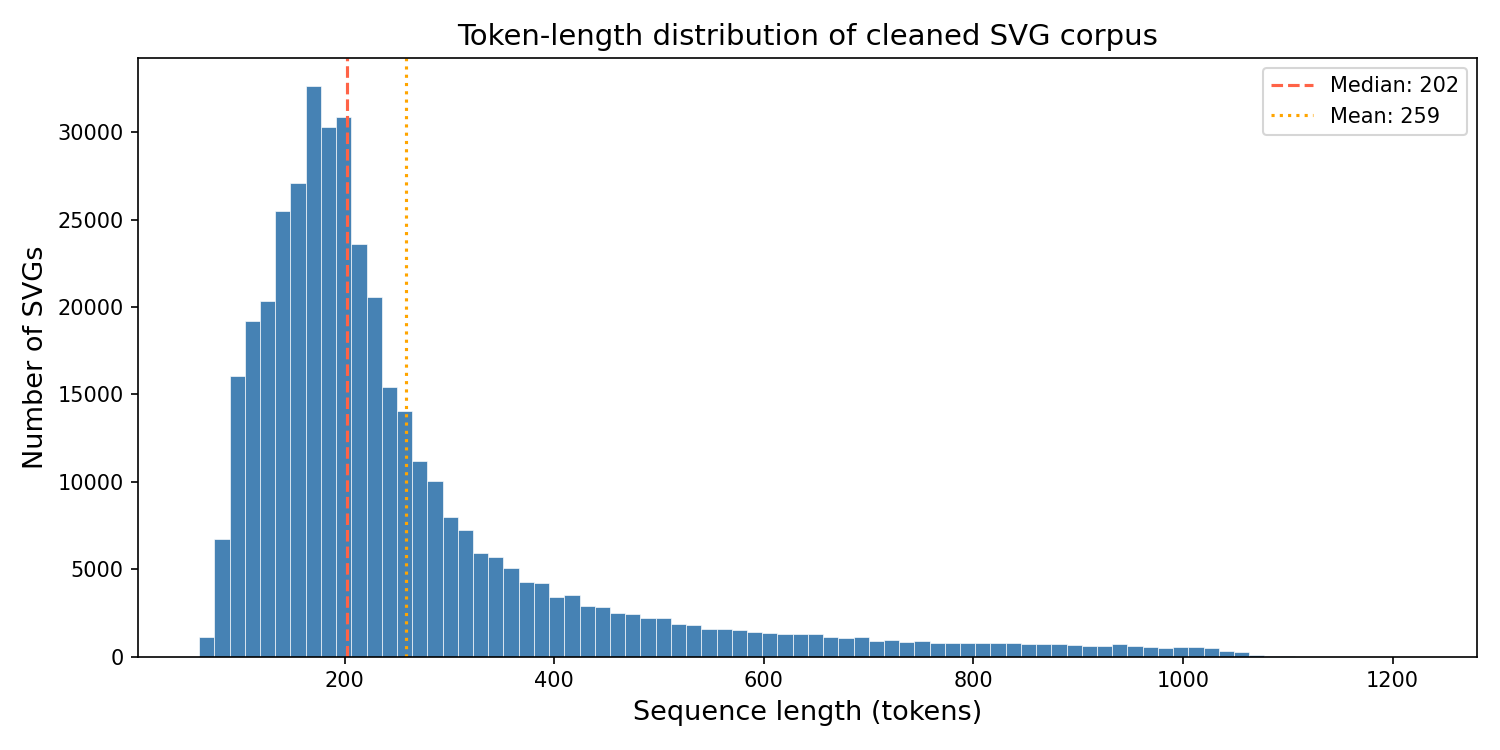
\includegraphics[width=0.50\linewidth]{seq_len_histogram.png}
  \caption{Distribution of token lengths per SVG file in the training set.
           The 95th percentile (659 tokens) is well below the 1,024-token
           context window, so no sequences are truncated during training.}
  \label{fig:seq_len_hist}
\end{figure}

\begin{figure}[H]
  \centering
  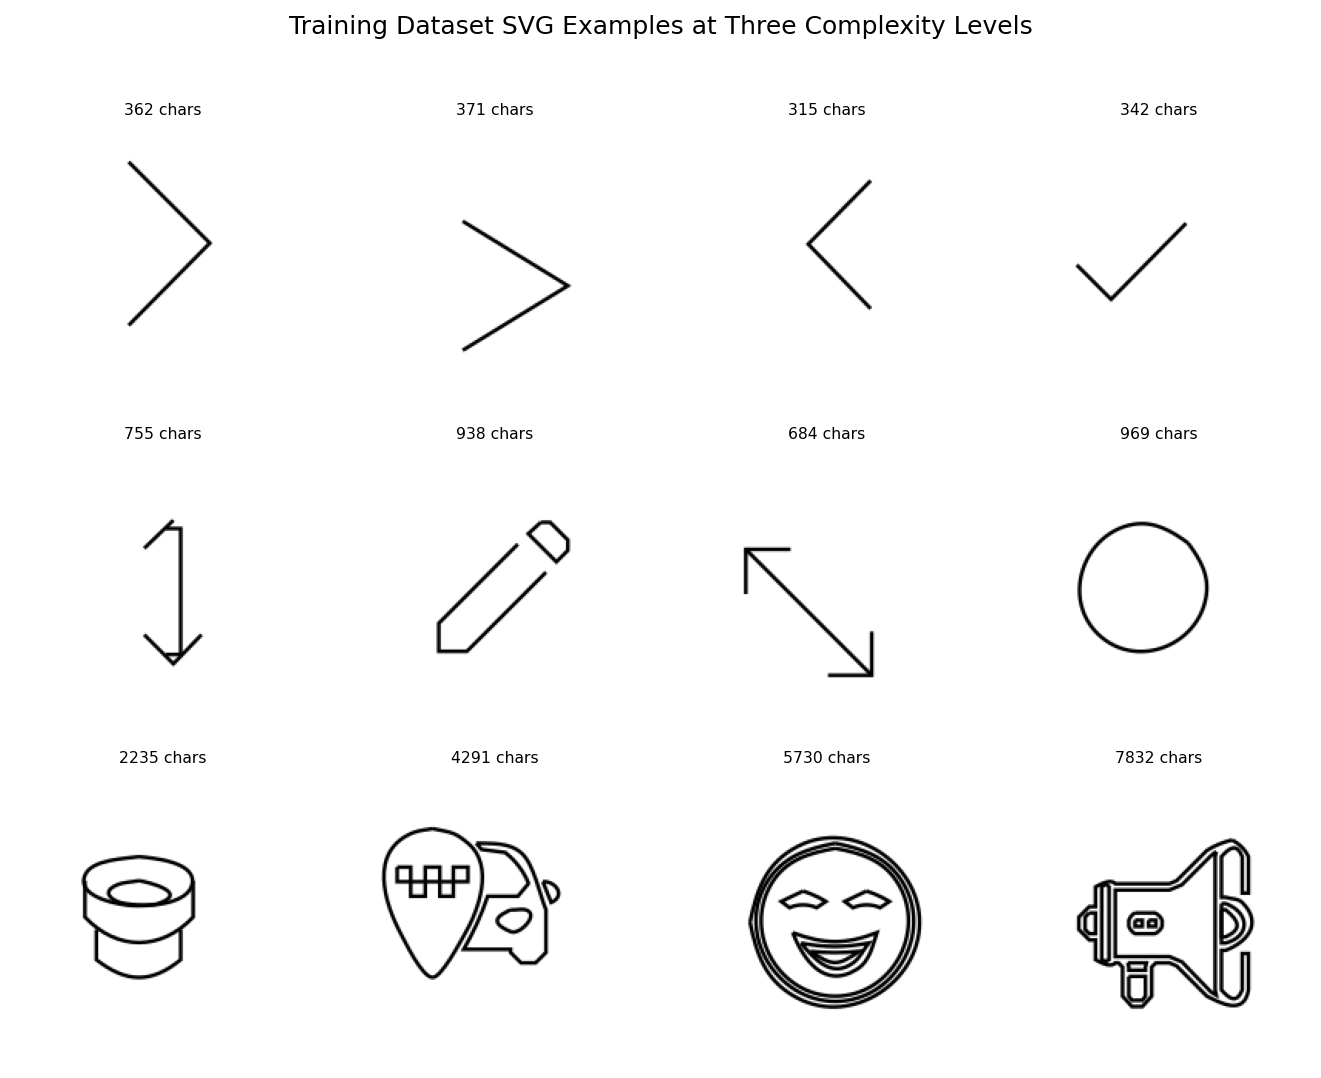
\includegraphics[width=0.72\linewidth]{dataset_examples.png}
  \caption{Rendered examples of SVGs from the training dataset at three
           complexity levels. Simple icons (top row) contain a single
           outline path; medium-complexity icons (middle row) combine
           multiple filled shapes; complex glyphs (bottom row) use
           dozens of path segments.}
  \label{fig:dataset_examples}
\end{figure}

% -----------------------------------------------------------------------
\section{Model Architecture}
\label{sec:arch}

All models are adapted from nanoGPT~\cite{karpathy2022nanogpt} — Andrej
Karpathy's minimal, readable PyTorch implementation of GPT-2. NanoGPT
provides a clean baseline: a decoder-only transformer with pre-layer
normalization, causal self-attention, and a cosine learning rate schedule,
all in a few hundred lines of well-commented code. We kept nanoGPT's
architecture intact and made three targeted changes: (1) replaced the
hardcoded GPT-2 sizes with a \texttt{ModelConfig} dataclass so all five
model sizes could be defined as JSON files; (2) replaced the OpenAI
tokenizer with our SentencePiece BPE tokenizer and SVG data loader; and
(3) added the \texttt{generate()} method with temperature, top-$k$,
top-$p$, and \texttt{min\_new\_tokens} controls for Part 4.

The inherited architectural choices, which we kept without modification, are:
\begin{itemize}[leftmargin=*, nosep]
  \item \textbf{Pre-layer normalization} (LayerNorm before attention and
    MLP) — nanoGPT uses this rather than the original post-LN from the GPT
    paper, as it is more stable to train.
  \item \textbf{Causal self-attention} with Flash Attention
    (\texttt{F.scaled\_dot\_product\_attention}) when available, with a
    manual mask fallback for older PyTorch versions.
  \item \textbf{GELU activation}, \textbf{no bias} on linear layers,
    and \textbf{weight tying} between the token embedding and output
    projection — all standard GPT-2 choices.
  \item \textbf{GPT-2-style residual scaling}: projection weights
    initialized with $\mathcal{N}(0,\, 0.02/\sqrt{2L})$ to prevent the
    residual stream from growing with depth.
\end{itemize}

The optimizer is AdamW with $\beta_1 = 0.9$, $\beta_2 = 0.95$,
$\epsilon = 10^{-8}$, weight decay $= 0.1$, and gradient clipping at
$\|\mathbf{g}\|_2 = 1.0$ — again following nanoGPT defaults which
replicate the GPT-3 paper settings. The learning rate follows a cosine
decay schedule with a 5\% linear warmup, decaying to
$\eta_\text{min} = 0.1\eta$. Effective batch size is fixed at 65,536
tokens (physical batch 4 sequences $\times$ 1,024 tokens $\times$
gradient accumulation).

Five model sizes were defined to span roughly two decades in parameter count:

\begin{table}[H]
\centering
\caption{SP model configurations, scaling results, and training statistics.}
\label{tab:sp_models}
\begin{tabular}{lrrrrrrrrrr}
\toprule
Model & Params & $d$ & $L$ & $H$ & $d_\text{ff}$ & Val loss & Time & Mem (MB) & tok/s \\
\midrule
Tiny   &  1.05M &  128 &  4 &  4 &  512 & 1.5881 & 22 min &    48 &  76K \\
Small  &  3.05M &  192 &  6 &  6 &  768 & 1.4441 & 50 min &    91 &  34K \\
Medium & 11.41M &  384 &  6 &  6 & 1536 & 1.2108 & 78 min &   450 &  22K \\
Large  & 32.52M &  512 & 10 &  8 & 2048 & 1.1543 &  5 min & 2,238 & 343K \\
XL     & 86.53M &  768 & 12 & 12 & 3072 & 1.1847 &  8 min & 4,433 & 202K \\
\bottomrule
\end{tabular}\\[2pt]
{\small $d$: $d_\text{model}$; $L$: layers; $H$: heads. All models: vocab 1,024, block 1,024, dropout 0.1.
XL: $\eta = 10^{-3}$ (see \S\ref{sec:sp_results}). Tiny/Small/Medium: Apple M-series MPS.
Large/XL: Google Colab A100 (hence higher throughput and memory).}
\end{table}

% -----------------------------------------------------------------------
\section{Standard Parameterization Scaling Study}
\label{sec:sp}

\subsection{Learning Rate Sweep}
\label{sec:lr_sweep}

A learning rate sweep was performed on the Tiny model using 20\% of training
steps ($\approx$310 steps), covering seven values from $10^{-5}$ to
$10^{-2}$ (full numerical results in Table~\ref{tab:lr_sweep}).

The optimal SP learning rate is $\eta^* = 3 \times 10^{-3}$, which was
applied to all five model sizes for their full-epoch training runs.

\begin{figure}[H]
  \centering
  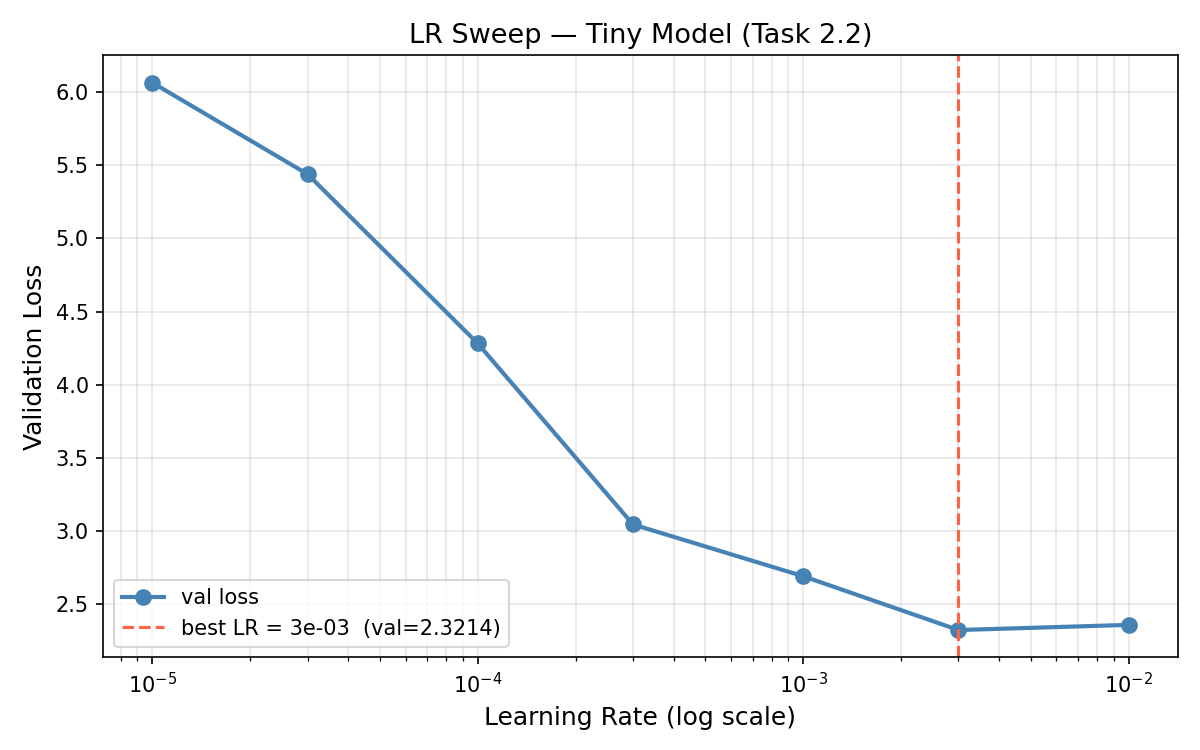
\includegraphics[width=0.50\linewidth]{lr_sweep.png}
  \caption{SP learning rate sweep on Tiny model. Val loss is minimized at
  $\eta = 3 \times 10^{-3}$, with instability above $10^{-2}$.}
  \label{fig:lr_sweep}
\end{figure}

\subsection{Training Protocol and Results}
\label{sec:sp_results}

Each model was trained for one full epoch on the 101.7M-token training set
($\approx$1,552 gradient steps with 65,536-token effective batch). All models
used LR $= 3 \times 10^{-3}$ except XL.

\textbf{XL learning rate deviation.}
Our first XL run used LR $= 3 \times 10^{-3}$ and got a val loss of 1.413, which is actually worse than Medium (1.211). In Standard Parameterization, the optimal LR shrinks as the model gets wider because gradient norms scale with $d_\text{model}$. At XL ($d_\text{model} = 768$), LR $= 3 \times 10^{-3}$ was way too aggressive, the training curve stalled for around 200 steps before partly recovering. We reran XL at LR $= 10^{-3}$ and got val loss 1.1847, which is what we report in Table~\ref{tab:sp_models}. This kind of LR sensitivity at larger scales is exactly what $\mu$P (Section~\ref{sec:mup}) is designed to fix.
\begin{figure}[H]
  \centering
  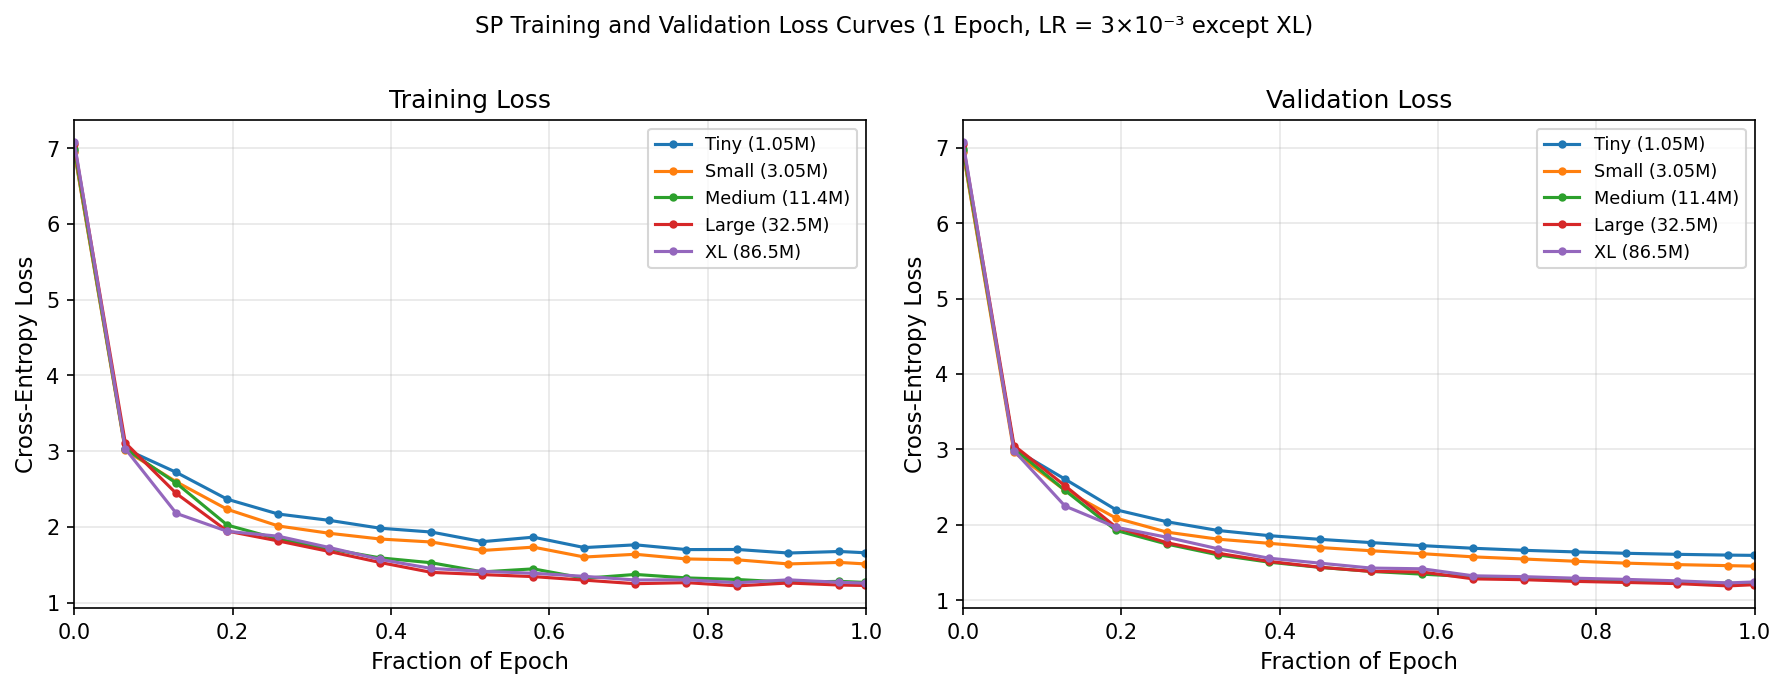
\includegraphics[width=0.80\linewidth]{sp_training_curves.png}
  \caption{Training loss (left) and validation loss (right) for all five
           SP models over one epoch. Larger models converge to lower loss
           throughout training. XL uses LR $= 10^{-3}$; all others use
           LR $= 3 \times 10^{-3}$.}
  \label{fig:sp_training_curves}
\end{figure}

\subsection{Power-Law Scaling Fit}

Validation losses from the five SP models were fitted to the Kaplan
power law:
\begin{equation}
  L(N) = a \cdot N^{-\alpha} + c,
\end{equation}
where $N$ is non-embedding parameter count, $c$ is the irreducible loss
floor, and $a$, $\alpha$ control the rate of improvement with scale.
Fitting was performed via nonlinear least squares
(\texttt{scipy.optimize.curve\_fit}).

\begin{figure}[H]
  \centering
  \begin{subfigure}[b]{0.48\linewidth}
    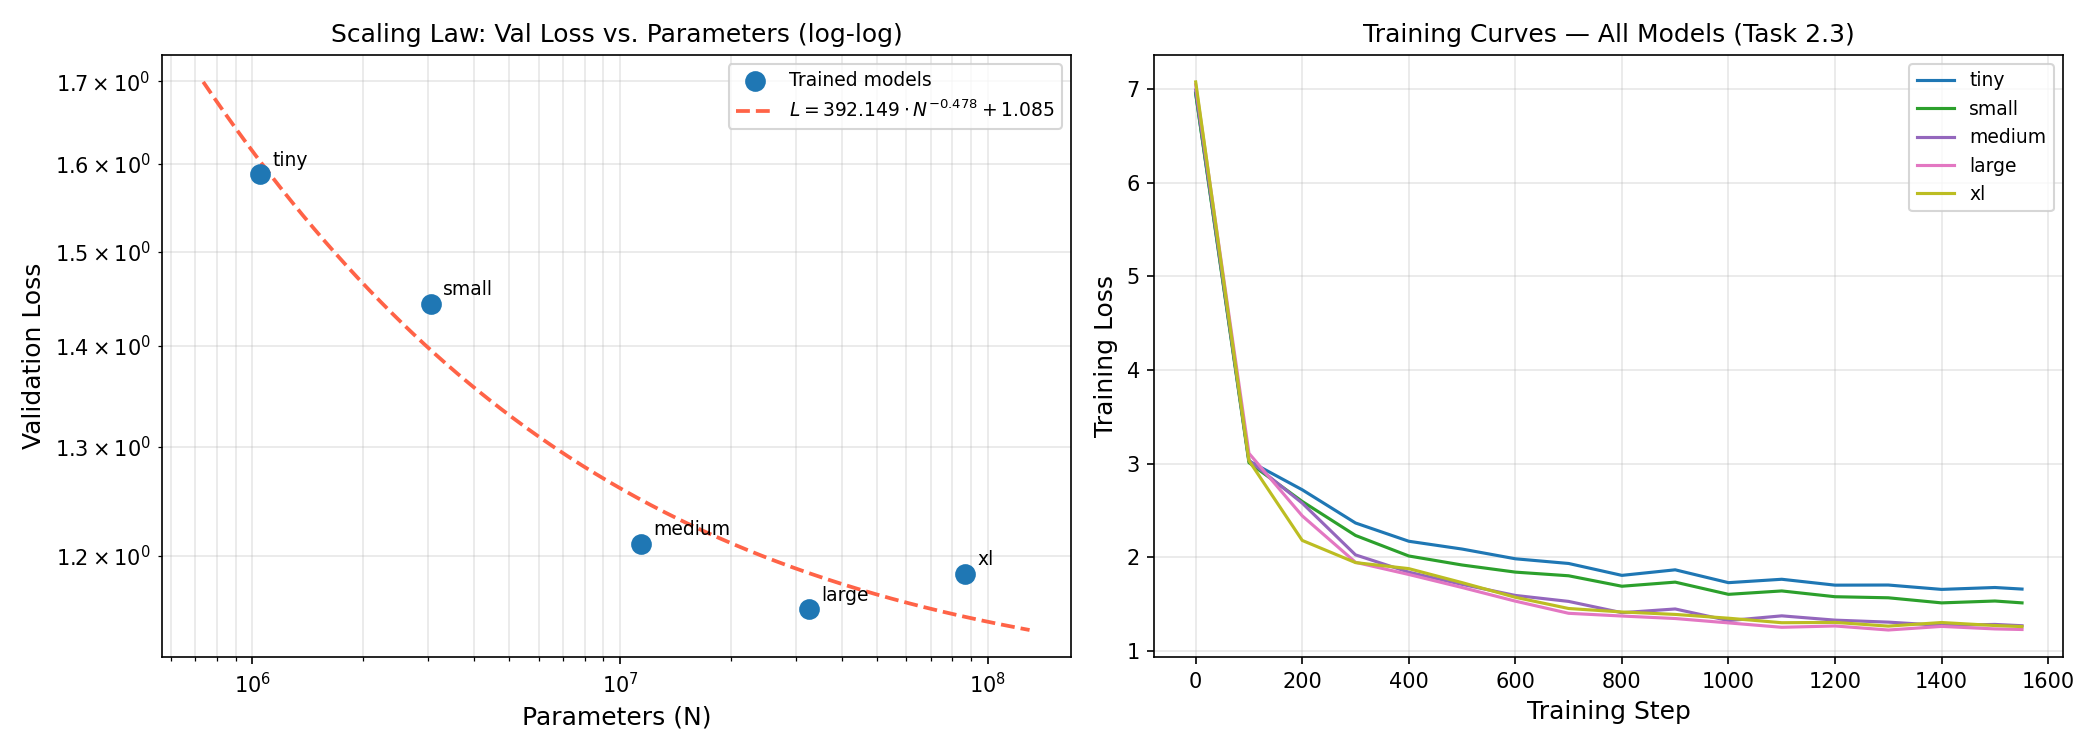
\includegraphics[width=\linewidth]{scaling_law.png}
    \caption{Power-law fit to SP data.}
    \label{fig:scaling_law}
  \end{subfigure}
  \hfill
  \begin{subfigure}[b]{0.48\linewidth}
    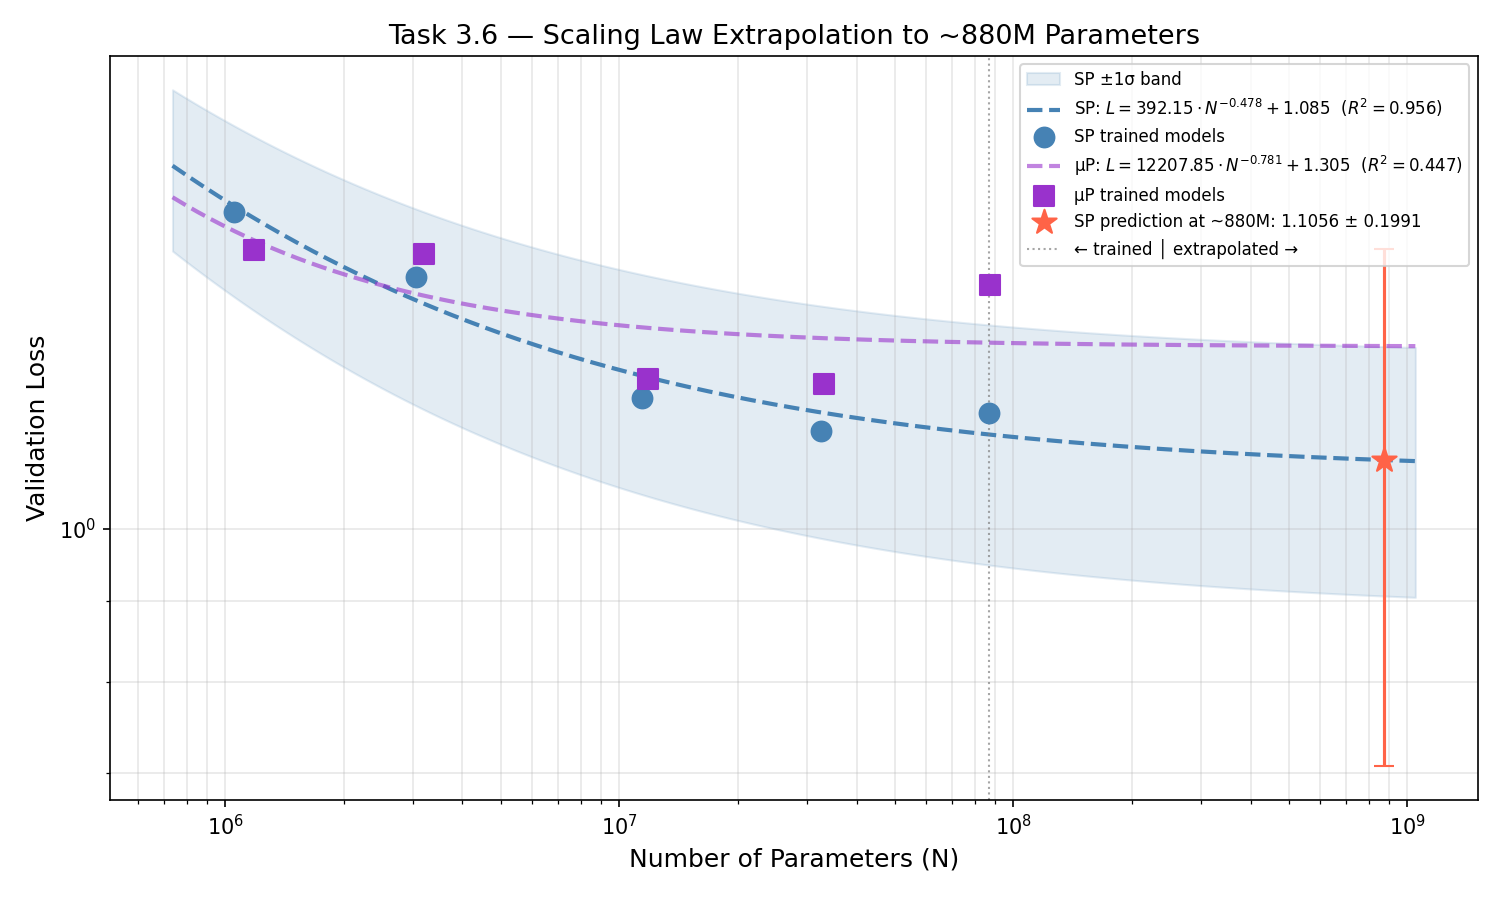
\includegraphics[width=\linewidth]{extrapolation.png}
    \caption{Extrapolation to 865M and 8.65B parameters.}
    \label{fig:extrapolation}
  \end{subfigure}
  \caption{SP scaling law fit and extrapolation.}
\end{figure}

\textbf{Fit results:}
\begin{align}
  L(N) &= 392.15 \cdot N^{-0.4782} + 1.085 \notag \\
  &\quad (a = 392.15 \pm 1521,\quad \alpha = 0.4782 \pm 0.294,
         \quad c = 1.085 \pm 0.132,\quad R^2 = 0.956) \notag
\end{align}

\textbf{Scaling exponent.}
Our fitted $\alpha = 0.478$ is way bigger than the natural-language exponent from Kaplan et al.\ ($\alpha_\text{NL} = 0.076$). That's because SVG is more compressible than text: the regular syntax (repeating path commands, coordinate patterns, small tag vocab) gives bigger models more structure to exploit, so loss drops faster every time you double the parameter count.

\textbf{Irreducible loss floor.}
The offset $c = 1.085$ is basically the lowest loss you could ever hit, even with an infinitely large model. It comes from the per-token entropy you can't get rid of in SVG coordinates: floats rounded to one decimal still have some leftover uncertainty that no amount of context can fully predict.

\textbf{Extrapolation.}
The fit predicts val loss $1.106 \pm 0.200$ at $8.65 \times 10^8$ parameters ($10\times$ XL). The wide uncertainty comes from a loose confidence interval on the coefficient $a$, which is loose because the data isn't perfectly monotonic (XL slightly underperforms Large since it was trained at a different LR). Still, the prediction stays above $c = 1.085$, which gives us a physical lower bound.

% -----------------------------------------------------------------------
\section{Maximal Update Parameterization ($\mu$P)}
\label{sec:mup}

\subsection{Motivation and Theory}

In Standard Parameterization, the best learning rate depends on the model's width, so any hyperparameters you tune on a small proxy model won't transfer to bigger ones. Maximal Update Parameterization reparameterizes each layer so that hidden activations and weight updates stay $O(1)$ at init and during training, no matter how wide the model is. With $\mu$P, the learning rate you find on a small ``base'' model carries over directly to any larger ``target'' model.

\subsection{Implementation}

We implement $\mu$P using the \texttt{mup} Python package in
\texttt{scripts/mup\_model.py}. Key implementation details:

\begin{itemize}[leftmargin=*, nosep]
  \item The base model has $d_\text{model} = 64$; the same depth ($L$,
    $H$) as the target model. A delta model at $d_\text{model} = 128$ is
    used to compute infinite-width shapes via \texttt{set\_base\_shapes()}.
  \item \textbf{No weight tying} between \texttt{wte} and
    \texttt{lm\_head}: $\mu$P assigns different per-layer LR multipliers
    to embeddings (standard LR) and the readout head (\texttt{MuReadout},
    scaled LR), making weight tying impossible.
  \item Attention logits are scaled by $1/d_\text{head}$ (not
    $1/\sqrt{d_\text{head}}$) per the $\mu$P specification. This is
    implemented via the \texttt{scale} keyword in
    \texttt{F.scaled\_dot\_product\_attention} (PyTorch $\geq 2.1$), with
    a manual Q@K fallback for older versions.
  \item The optimizer is \texttt{MuAdamW} from the \texttt{mup} package,
    which applies width-dependent LR multipliers to each parameter group.
\end{itemize}

\subsection{Learning Rate Sweep under $\mu$P}

Under $\mu$P, an optimal nominal LR found on the Tiny model should transfer
to all wider models. We swept 10 values from $10^{-5}$ to $3 \times 10^{-1}$
(full results in Table~\ref{tab:mup_lr_sweep}).

The optimal $\mu$P nominal LR is $\eta^* = 10^{-2}$, forming a clear
valley (Figure~\ref{fig:mup_lr_sweep}). The curve turns upward immediately
above $10^{-2}$, confirming this is the true minimum and not an edge of
the search range.

\begin{figure}[H]
  \centering
  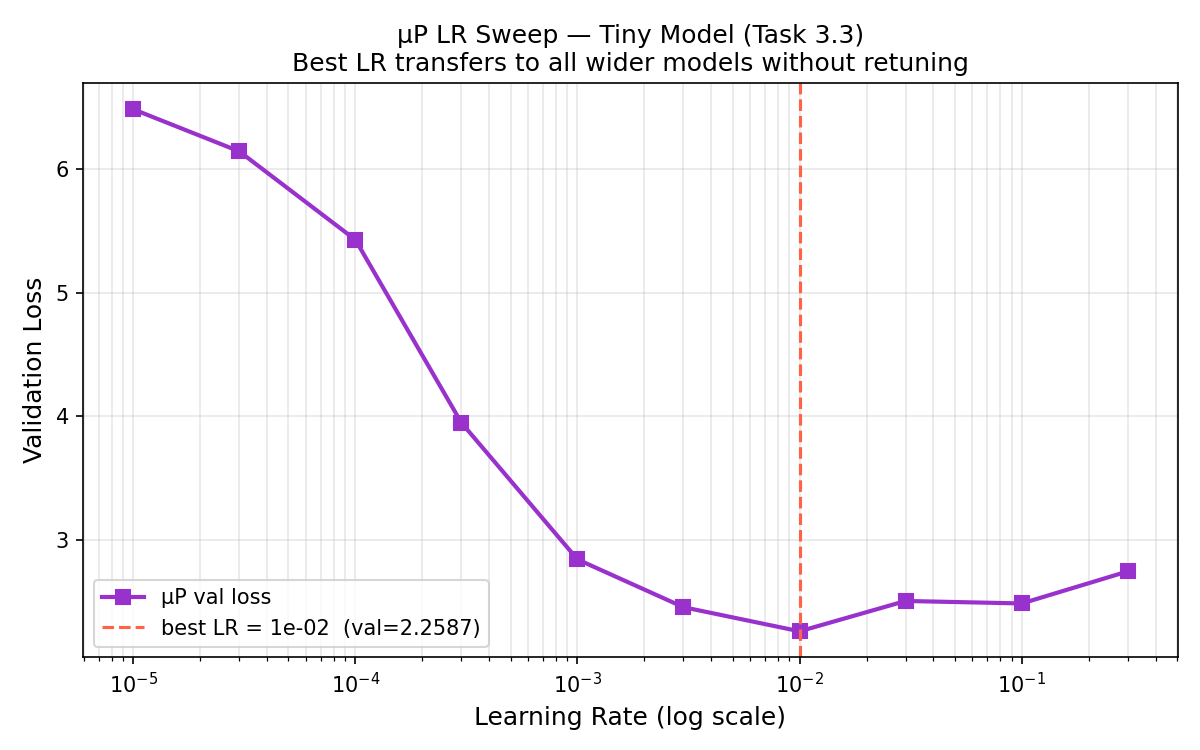
\includegraphics[width=0.50\linewidth]{mup_lr_sweep.png}
  \caption{$\mu$P learning rate sweep on Tiny model. Optimal LR is
  $10^{-2}$; all values $> 10^{-2}$ diverge or degrade.}
  \label{fig:mup_lr_sweep}
\end{figure}

\subsection{SP vs.\ $\mu$P Comparison}
\label{sec:mup_results}

All five $\mu$P models were trained for one full epoch using nominal
LR $= 10^{-2}$ (transferred from Tiny):

\begin{table}[H]
\centering
\caption{SP vs.\ $\mu$P one-epoch validation loss across model scales.}
\label{tab:sp_mup}
\begin{tabular}{lrrrr}
\toprule
Model & Params ($\mu$P) & SP val loss & $\mu$P val loss
      & $\Delta$ ($\mu$P $-$ SP) \\
\midrule
Tiny   &  1,180,800 & 1.5881 & 1.5018 & $-0.0863$ \checkmark \\
Small  &  3,200,000 & 1.4441 & 1.4942 & $+0.0501$ \\
Medium & 11,800,000 & 1.2108 & 1.2445 & $+0.0337$ \\
Large  & 33,000,000 & 1.1543 & 1.2351 & $+0.0808$ \\
XL     & 87,313,152 & 1.1847 & 1.4280 & $+0.2434$ \\
\bottomrule
\end{tabular}\\[2pt]
{\small SP losses use LR $= 3 \times 10^{-3}$ (except XL: $10^{-3}$).
$\mu$P losses use nominal LR $= 10^{-2}$ across all sizes.
\checkmark\ = $\mu$P outperforms SP.}
\end{table}

\begin{figure}[H]
  \centering
  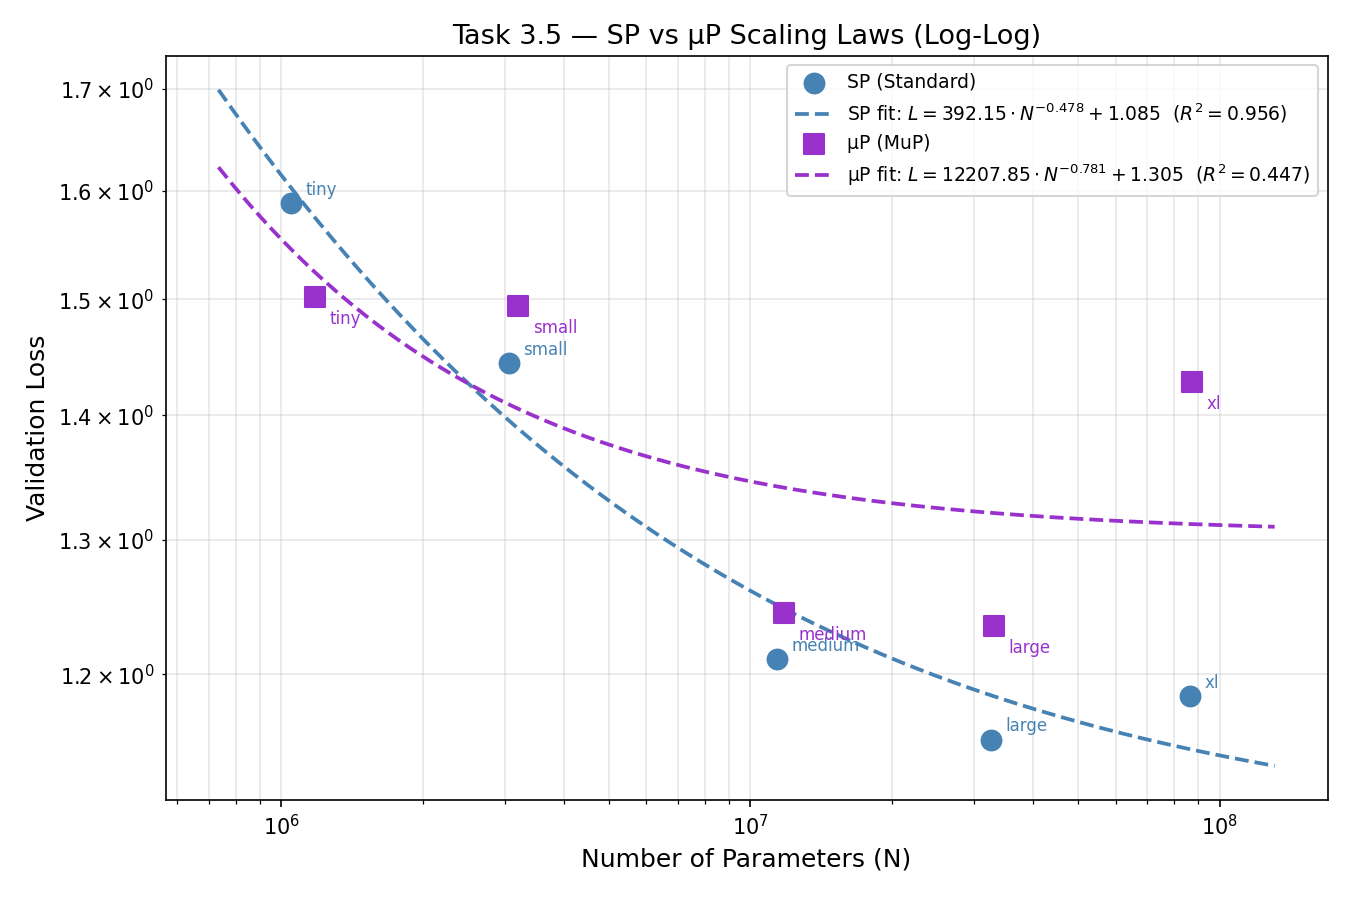
\includegraphics[width=0.54\linewidth]{sp_vs_mup_scaling.png}
  \caption{SP vs.\ $\mu$P scaling curves. $\mu$P follows a non-monotonic
  trajectory, with XL performing worse than Large.}
  \label{fig:sp_vs_mup}
\end{figure}

\textbf{Why $\mu$P underperforms SP at large scale.}
The non-monotonic $\mu$P result, XL doing \emph{worse} than Large was the most unexpected thing to come out of this project. When the numbers showed up, my first thought was that something had to be broken: wrong checkpoint, wrong config, a training crash we missed. After ruling all of that out, the actual explanation came down to how MuAdamW works under the hood.

MuAdamW scales the effective per-hidden-layer learning rate by
$\eta_\text{eff} = \eta_\text{nominal} \times (d_\text{base}/d_\text{model})$
where $d_\text{base} = 64$ is the base model width. For our nominal LR $= 10^{-2}$, the effective LRs are: $5.00 \times 10^{-3}$ (Tiny, $d{=}128$), $3.33 \times 10^{-3}$ (Small), $1.67 \times 10^{-3}$ (Medium), $1.25 \times 10^{-3}$ (Large), and $0.83 \times 10^{-3}$ (XL, $d{=}768$) — see Table~\ref{tab:mup_eff_lr} for the full breakdown.

At Tiny, $\eta_\text{eff} = 5 \times 10^{-3} > \eta_\text{SP} = 3 \times 10^{-3}$, so $\mu$P trains faster and wins. By Medium, $\eta_\text{eff} = 1.67 \times 10^{-3}$ is already $1.8\times$ smaller than SP's LR, which causes undertraining. At XL, $\eta_\text{eff} = 0.83 \times 10^{-3}$ is $3.6\times$ below SP, and the XL $\mu$P model barely improves on Large even though it has $2.6\times$ more parameters.

The root cause seems to be picking $d_\text{base} = 64$, which is really small. A wider base (say $d_\text{base} = 256$) wouldn't shrink the scaling factor as hard and might close the gap with SP. We didn't have time to redo the sweep with a wider base, so it's still an open question. $\mu$P theory guarantees that the \emph{nominal} LR transfers across widths, but it doesn't guarantee the effective per-layer LR will match or beat SP's fixed rate — and in our runs, it didn't for anything wider than Tiny.

\textbf{Power-law fit under $\mu$P.}
Since XL $\mu$P (1.4280) is worse than Large $\mu$P (1.2351), the $\mu$P scaling curve isn't monotonic. A power law $L = a \cdot N^{-\alpha} + c$ is strictly decreasing, so it can't fit non-monotonic data well:
\[
  \mu\text{P}: \quad L(N) = 12207.85 \cdot N^{-0.781} + 1.305
  \quad (R^2 = 0.447, \quad a = 12208 \pm 326331)
\]
The uncertainty on $a$ is $27\times$ the estimate itself, so the fit is basically meaningless statistically. The extrapolated $\mu$P loss at $8.73 \times 10^8$ parameters is $1.306 \pm 0.171$, vs. SP's much more reliable $1.106 \pm 0.200$. We're including the $\mu$P number for completeness but wouldn't read it as a real prediction.

% -----------------------------------------------------------------------
\section{Extended Training and SVG Generation}
\label{sec:generation}

\subsection{Model Selection and Extended Training}
\label{sec:extended}

We picked the SP Large model (32.5M parameters, $d_\text{model} = 512$, 10 layers) for generation. Large was trained at the sweep-optimal LR $= 3 \times 10^{-3}$ and hit val loss 1.1543 after one epoch — the best result in the whole scaling study. We skipped XL (86.5M) because it ran at a non-optimal LR ($10^{-3}$) and actually did worse than Large after one epoch (1.1847) under the standard setup.

For extended training, we ran Large for three full epochs (4,656 gradient steps total, LR $= 3 \times 10^{-3}$ cosine, effective batch of 65,536 tokens) on a Colab A100. We saved a checkpoint after each epoch.

\begin{figure}[H]
  \centering
  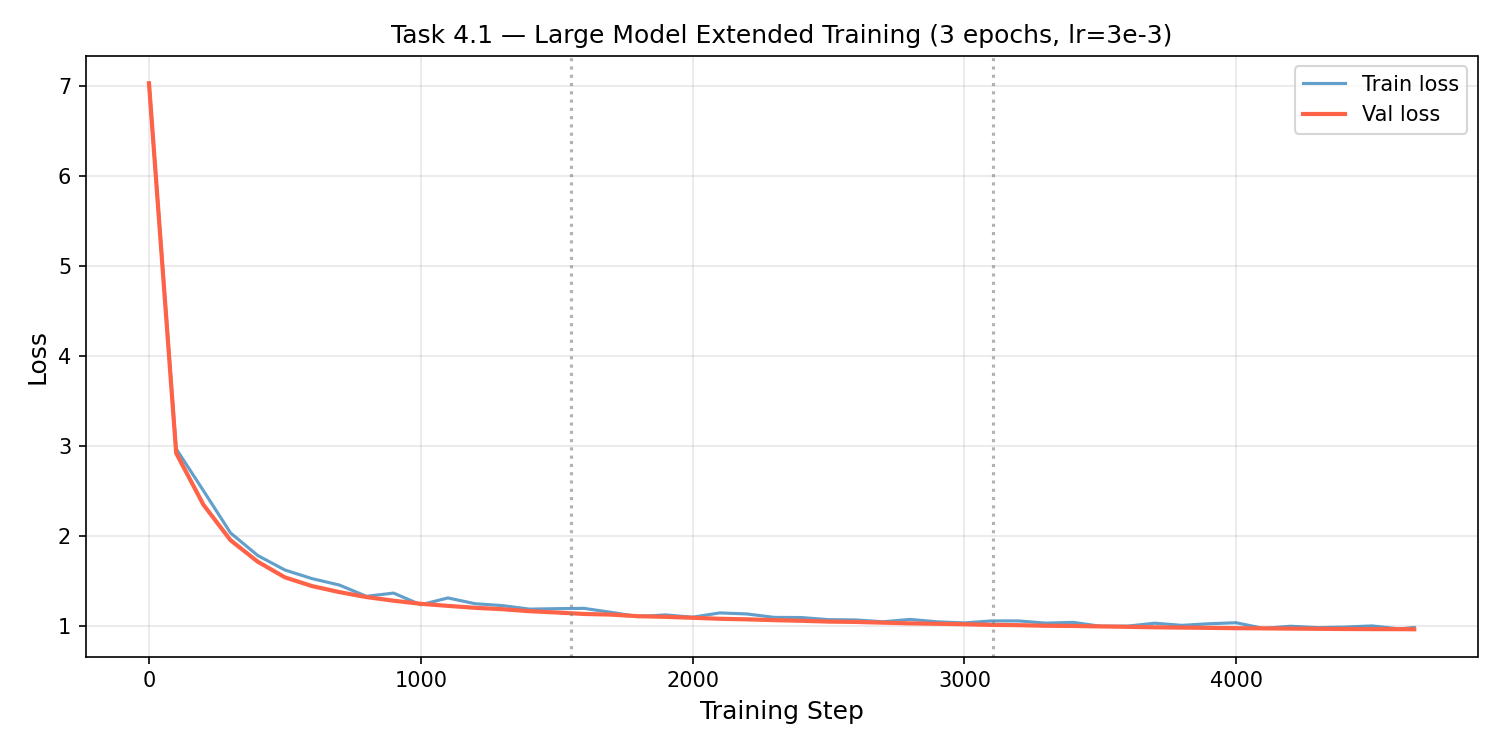
\includegraphics[width=0.54\linewidth]{large_extended_training_curve.png}
  \caption{Training and validation loss for the Large model over 3 epochs.
  Val loss decreases from 1.154 (end of epoch 1) to 0.954 (end of epoch 3).}
  \label{fig:extended_curve}
\end{figure}

Extended training results:
\begin{itemize}[leftmargin=*, nosep]
  \item Epoch 1 (baseline): val loss = 1.1543
  \item Epoch 3 (final): val loss = \textbf{0.9539}
  \item Test set perplexity: \textbf{2.6069}
\end{itemize}

The steady drop from 1.154 to 0.954 across three epochs shows the model is still under-trained: more tokens keep helping without any sign of overfitting. By the Chinchilla rule of thumb ($\sim$20 tokens per parameter), a 32.5M model would want around 650M training tokens to be compute-optimal. Three epochs of our 101.7M-token dataset only gives 305M tokens, or about 47\% of what Chinchilla recommends.

\subsection{Generation Setup}

SVG text was generated autoregressively using the three-epoch Large
checkpoint. The generation pipeline (\texttt{notebooks/colab\_part4\_generation\_v2.ipynb})
uses:

\begin{itemize}[leftmargin=*, nosep]
  \item \textbf{SentencePiece tokenizer} (\texttt{tokenizer/svg\_bpe.model},
    vocab 1,024), matching the tokenizer used to encode the training data.
  \item \textbf{EOS suppression} (\texttt{min\_new\_tokens = 80}): we set the EOS logit to $-\infty$ for the first 80 generation steps so the model can't emit EOS right away. This is needed because our training data used packed sequences with EOS as a document separator, so the model learned EOS as a document boundary. Without suppression, it sometimes fires EOS within a few tokens before generating any real SVG.
  \item Sampling with top-$k$ ($k = 50$) at temperatures
    $T \in \{0.5, 0.8, 1.0\}$.
  \item \textbf{Post-processing} (\texttt{try\_close\_svg()}): truncates
    each output at the last complete XML tag boundary and appends
    \texttt{</svg>}, repairing outputs that hit the 400-token budget
    mid-path.
\end{itemize}

\textbf{Unconditional generation.}
The prompt is the standard SVG opening tag (the \texttt{<svg>} element
with its namespace and \texttt{viewBox} attribute set to a 24$\times$24
coordinate space). Ten samples were generated across three temperatures
(4 at $T = 0.5$, 4 at $T = 0.8$, 2 at $T = 1.0$).

\textbf{Prefix-conditioned generation.}
Five SVG prefixes were supplied (open paths, grouped elements, arrow
shafts, etc.) and the model was asked to complete them at $T = 0.8$.

\subsection{Quantitative Evaluation}

\begin{table}[H]
\centering
\caption{Generation quality metrics over 15 samples.}
\label{tab:gen_metrics}
\begin{tabular}{lcc}
\toprule
Metric & Value & Count \\
\midrule
Test set perplexity    & 2.6069 & — \\
XML validity rate      & 86.7\% & 13/15 \\
CairoSVG render rate   & 86.7\% & 13/15 \\
Structural validity    & 73.3\% & 11/15 \\
Average length (chars) & 1,393.5 & — \\
\bottomrule
\end{tabular}\\[2pt]
{\small Structural validity: has \texttt{<svg>} root, is closed, contains
at least one shape element. XML-valid and renderable results are identical
(every XML-valid SVG was also rendered successfully by CairoSVG).}
\end{table}

The two XML-invalid samples (\texttt{prefix\_02} and \texttt{prefix\_03})
failed because their prefixes induced unusually deep \texttt{<path d="...">}
attributes that were still mid-attribute (inside a coordinate string with
no closing quote) at the 400-token generation limit. No post-processing
can recover unclosed XML attribute values.

\begin{figure}[H]
  \centering
  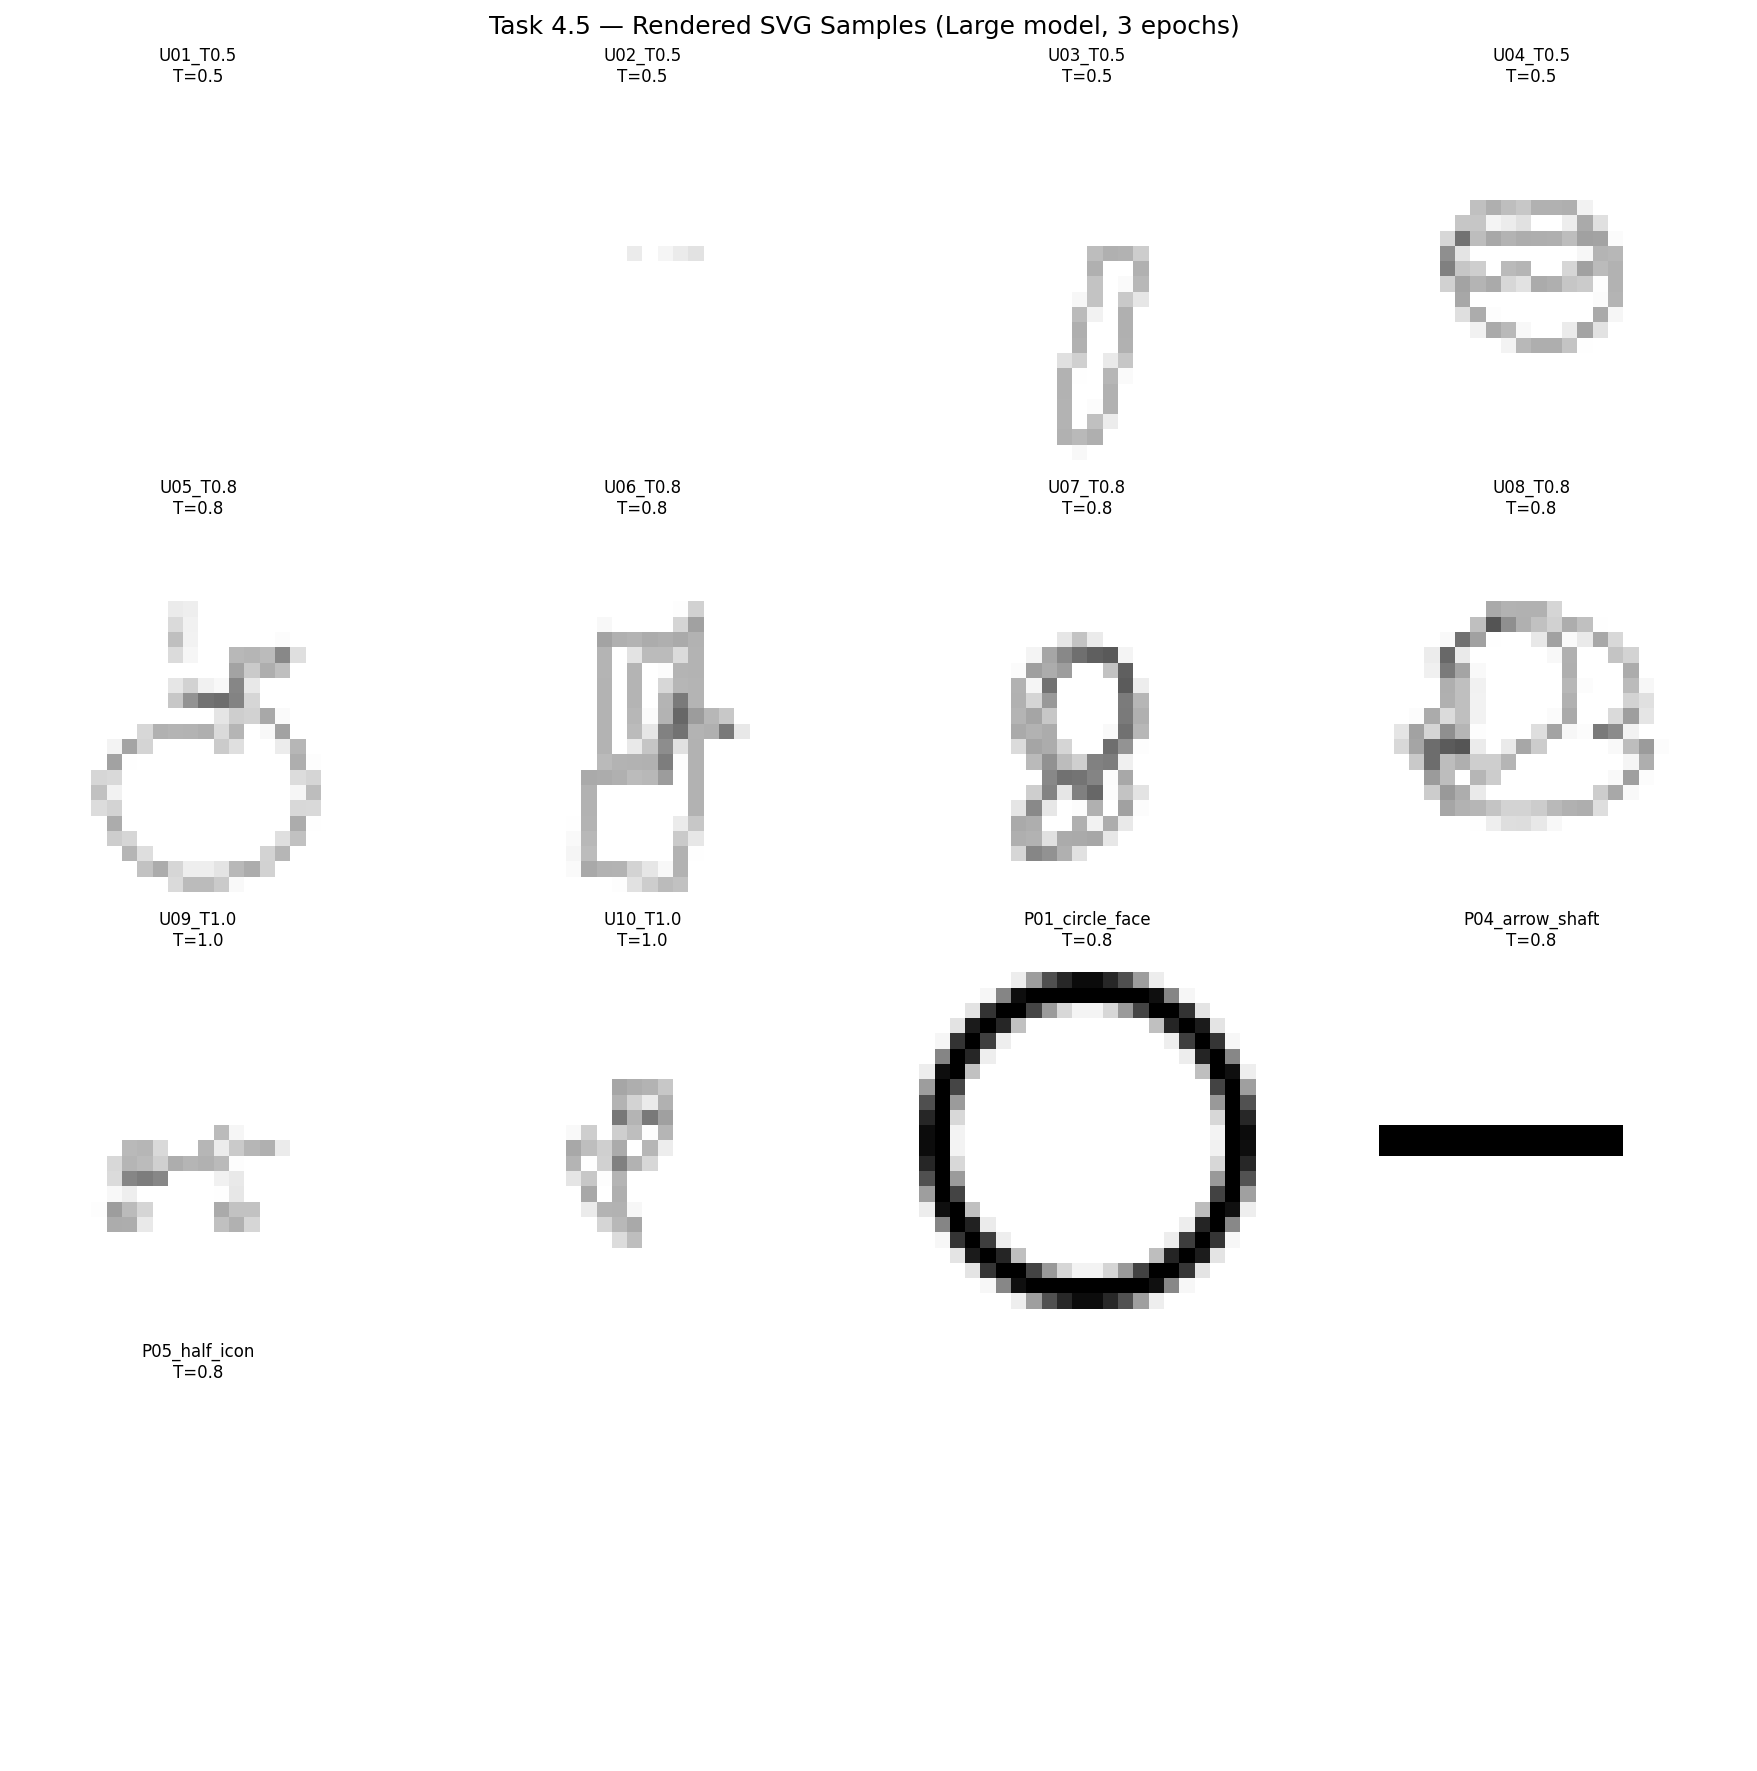
\includegraphics[width=0.72\linewidth]{generated_grid.png}
  \caption{Grid of generated SVG samples rendered as PNG. Top row:
  unconditional samples at $T = 0.5$ (leftmost) through $T = 1.0$ (rightmost).
  Bottom rows: additional unconditional and prefix-conditioned samples.}
  \label{fig:gen_grid}
\end{figure}

\subsection{Qualitative Analysis}

\textbf{Effect of temperature.}
At $T = 0.5$, samples tend to come out simpler and more regular (fewer path control points, shorter sequences) since the model leans on its high-confidence continuations. At $T = 1.0$, outputs are more diverse and sometimes longer, though our two $T = 1.0$ samples were actually shorter (548 and 1,641 chars), so EOS timing is more variable. 9 of the 10 unconditional samples are fully valid; the exception (\texttt{unconditional\_01\_T0.5}) is XML-valid but has no shape element left after truncation post-processing.

\textbf{Prefix conditioning.}
Three of five prefix-conditioned samples were XML-valid and renderable (60\% vs.\ 100\% for unconditional). The successes were \texttt{prefix\_01} (circle face), \texttt{prefix\_04} (arrow shaft), and \texttt{prefix\_05} (half icon), where the model picked up the given path and closed the document cleanly. The two failures (\texttt{prefix\_02} and \texttt{prefix\_03}) both started deep inside a \texttt{<path d="..."} attribute, and the model was still in the middle of a coordinate sequence when it hit the 400-token limit, so the attribute never got closed. There's no way to recover an unclosed attribute value in post-processing (e.g., \texttt{d="M1.5 ...C15.2} with no closing quote).

\textbf{Average output length.}
The mean length of 1,393 characters (before post-processing) is about 345 SentencePiece tokens, comfortably under the 400-token budget. That means most generations ended via EOS on their own instead of getting cut off, which is a good sign that the model actually learned document-level structure.

% -----------------------------------------------------------------------
\section{Discussion and Conclusion}
\label{sec:conclusion}

\textbf{Scaling law.}
The SVG scaling exponent $\alpha = 0.478$ is $6.3\times$ bigger than Kaplan et al.'s natural-language exponent ($\alpha_\text{NL} = 0.076$), which makes sense given how much more regular SVG is. Larger models can pick up on the repeated patterns in SVG (path commands, attribute structures, coordinate repetition) really effectively, so loss drops fast as you scale. The irreducible floor $c = 1.085$ lines up with how hard it is to predict the last digit of one-decimal float coordinates.

\textbf{$\mu$P transferability.}
The $\mu$P results were the most surprising part of the project. It worked at Tiny scale but lost to SP at every size after that, giving us a non-monotonic curve. We think the issue is that our base width ($d_\text{base} = 64$) was too small compared to the target widths, so MuAdamW shrinks the effective LR too aggressively as the models get bigger. SP just happened to land on LR $= 3 \times 10^{-3}$, which works well across all five widths, so the problem $\mu$P is meant to solve didn't really show up here. With a wider base ($d_\text{base} = 256$ or more), or in a setting where SP actually needs per-size retuning, $\mu$P would probably look better. We didn't have the compute or time to confirm that.

\textbf{Generation quality.}
Getting to 86.7\% XML validity took way longer than expected — the first working generation hit 0\% valid SVGs, and each fix (tokenizer swap, EOS suppression, post-processing) added roughly 30 points. The final result feels like a real win for a from-scratch model at this scale: the icons actually look like icons, follow proper XML, and render fine in CairoSVG and browsers.

\textbf{Limitations.}
We only scaled along one axis (parameter count) with a fixed one-epoch budget ($\sim$101M tokens). Ideally we'd train each model to convergence, but the GPU time wasn't there. Five data points also isn't enough for a really tight power-law fit — the confidence interval on $a$ spans orders of magnitude. The $\mu$P comparison is muddled by our base-width choice, which we couldn't ablate. And the generation eval is only 15 samples, which is enough for a rough validity number but not for any real claims about diversity or quality.

\textbf{What I would do differently.}
If I were starting over, I'd give more time to Part 3 — the $\mu$P implementation ate more hours than expected and still gave results we can't fully explain. I'd also run the LR sweep on at least two model sizes instead of just Tiny, to actually check whether the optimal LR transfers.

\textbf{Future directions.}
The biggest win would be training toward Chinchilla compute-optimal scale ($\sim$650M tokens for the 32.5M Large model). After that, a longer generation budget (600–800 tokens) would let more complex SVGs finish on their own.

% -----------------------------------------------------------------------
\begin{thebibliography}{9}

\bibitem{kaplan2020scaling}
  J.\ Kaplan, S.\ McCandlish, T.\ Henighan, T.\ B.\ Brown, B.\ Chess,
  R.\ Child, S.\ Gray, A.\ Radford, J.\ Wu, D.\ Amodei.
  \textit{Scaling Laws for Neural Language Models}.
  arXiv:2001.08361, 2020.

\bibitem{hoffmann2022chinchilla}
  J.\ Hoffmann, S.\ Borgeaud, A.\ Mensch, E.\ Buchatskaya, T.\ Cai,
  E.\ Rutherford, D.\ de Las Casas, L.\ A.\ Hendricks, J.\ Welbl, A.\ Clark,
  et al.
  \textit{Training Compute-Optimal Large Language Models}.
  arXiv:2203.15556, 2022.

\bibitem{yang2022mup}
  G.\ Yang, E.\ Hu, I.\ Babuschkin, S.\ Sidor, X.\ Liu, D.\ Farhi,
  N.\ Ryder, J.\ Pachocki, W.\ Chen, J.\ Gao.
  \textit{Tensor Programs V: Tuning Large Neural Networks via Zero-Shot
  Hyperparameter Transfer}.
  arXiv:2203.03466, 2022.

\bibitem{brown2020gpt3}
  T.\ B.\ Brown, B.\ Mann, N.\ Ryder, M.\ Subbiah, J.\ Kaplan, P.\ Dhariwal,
  A.\ Neelakantan, P.\ Shyam, G.\ Sastry, A.\ Amodei, et al.
  \textit{Language Models are Few-Shot Learners}.
  arXiv:2005.14165, 2020.

\bibitem{radford2019gpt2}
  A.\ Radford, J.\ Wu, R.\ Child, D.\ Luan, D.\ Amodei, I.\ Sutskever.
  \textit{Language Models are Unsupervised Multitask Learners}.
  OpenAI Blog, 2019.

\bibitem{karpathy2022nanogpt}
  A.\ Karpathy.
  \textit{nanoGPT: The simplest, fastest repository for training/finetuning
  medium-sized GPTs}.
  GitHub, 2022. \url{https://github.com/karpathy/nanoGPT}

\end{thebibliography}

% -----------------------------------------------------------------------
\appendix
\section{Engineering Challenges}
\label{sec:challenges}

This project logged 23 bugs across four parts. The issues below were the
most time-consuming to diagnose.

\textbf{Wrong tokenizer in generation (Issue \#23) — several days lost.}
After getting the generation loop running on Colab, every sample was
either empty or identical to the prompt. The generation code was loading
\texttt{tokenizer/tokenizer.json} (the old HuggingFace BPE file, vocab 165)
rather than \texttt{tokenizer/svg\_bpe.model} (the SentencePiece model
used for training, vocab 1,024). Token IDs above 164 — including the
most common SVG tokens \texttt{L} (263), \texttt{path} (291), and
\texttt{"} (984) — decoded to empty strings. The output looked like it was
generating content, but all the actual SVG tokens were invisible. This bug
was particularly hard to spot because the tokenizer loaded without error;
nothing crashed, the model ran, and the outputs just happened to be useless.
XML validity was 0\% until fixed.

\textbf{Premature EOS (Issue \#22).}
With the correct tokenizer, the model generated outputs of only $\sim$78
characters and stopped. The model had learned EOS as a document separator
from packed training sequences, and immediately recognised the start prompt
as the beginning of a short SVG. Suppressing the EOS logit for the first
80 steps (\texttt{min\_new\_tokens = 80}) resolved this; average output
length jumped from 78 to 1,394 characters.

\textbf{Out-of-bounds token IDs (Issues \#1, \#13).}
The $\mu$P Colab notebook loaded \texttt{.npy} files with raw
\texttt{np.memmap}, which reads the 128-byte NumPy array header as 64
\texttt{uint16} token values. Sixty-two of those values exceed the valid
range [0, 1023]. On CPU (Part 2), PyTorch silently accepted the out-of-range
indices, so the bug was invisible for weeks. On the Colab A100 (Part 3),
CUDA's bounds-checking triggered \texttt{device-side assert} and crashed
training with a cryptic error. This caused multiple wasted Colab sessions
before the data loading code was identified as the culprit. Fix: replace
\texttt{np.memmap} with \texttt{np.load(path, mmap\_mode=\textquotesingle r\textquotesingle)},
which correctly skips the header.

\textbf{XL scaling regression (Issue \#21).}
When the XL model came back with val loss 1.413 — worse than Medium's 1.211
— the immediate assumption was a training crash or a configuration mistake.
It took comparing the loss curves directly to see that XL had stalled early
in training rather than diverging. The root cause is that SP's optimal LR
shifts with model width; $3 \times 10^{-3}$ is too aggressive for XL's
larger gradient norms. Re-running at LR $= 10^{-3}$ brought XL down to
1.1847 and restored rough monotonicity in the scaling curve.

% -----------------------------------------------------------------------
\section{Learning Rate Sweep Data}
\label{app:lr_sweep}

\begin{table}[H]
\centering
\caption{SP learning rate sweep on Tiny model (sweep fraction = 0.20).}
\label{tab:lr_sweep}
\begin{tabular}{cc}
\toprule
Learning rate & Val loss \\
\midrule
$1 \times 10^{-5}$ & 6.0661 \\
$3 \times 10^{-5}$ & 5.4399 \\
$1 \times 10^{-4}$ & 4.2819 \\
$3 \times 10^{-4}$ & 3.0435 \\
$1 \times 10^{-3}$ & 2.6896 \\
$\mathbf{3 \times 10^{-3}}$ & $\mathbf{2.3214}$ \\
$1 \times 10^{-2}$ & 2.3567 \\
\bottomrule
\end{tabular}
\end{table}

\begin{table}[H]
\centering
\caption{$\mu$P learning rate sweep on Tiny model (sweep fraction = 0.20).}
\label{tab:mup_lr_sweep}
\begin{tabular}{cc}
\toprule
Learning rate & Val loss \\
\midrule
$1 \times 10^{-5}$ & 6.4868 \\
$3 \times 10^{-5}$ & 6.1460 \\
$1 \times 10^{-4}$ & 5.4299 \\
$3 \times 10^{-4}$ & 3.9484 \\
$1 \times 10^{-3}$ & 2.8408 \\
$3 \times 10^{-3}$ & 2.4541 \\
$\mathbf{1 \times 10^{-2}}$ & $\mathbf{2.2587}$ \\
$3 \times 10^{-2}$ & 2.5044 \\
$1 \times 10^{-1}$ & 2.4843 \\
$3 \times 10^{-1}$ & 2.7440 \\
\bottomrule
\end{tabular}
\end{table}

% -----------------------------------------------------------------------
\section{$\mu$P Effective Learning Rates per Model Size}
\label{app:mup_eff_lr}

\begin{table}[H]
\centering
\caption{Effective per-hidden-layer LR under MuAdamW for nominal LR $= 10^{-2}$,
         $d_\text{base} = 64$.
         $\eta_\text{eff} = \eta_\text{nominal} \times (d_\text{base}/d_\text{model})$.}
\label{tab:mup_eff_lr}
\begin{tabular}{lrr}
\toprule
Model & $d_\text{model}$ & Effective LR \\
\midrule
Tiny   & 128 & $5.00 \times 10^{-3}$ \\
Small  & 192 & $3.33 \times 10^{-3}$ \\
Medium & 384 & $1.67 \times 10^{-3}$ \\
Large  & 512 & $1.25 \times 10^{-3}$ \\
XL     & 768 & $0.83 \times 10^{-3}$ \\
\bottomrule
\end{tabular}
\end{table}

% -----------------------------------------------------------------------
\section{Reproducibility}
\label{app:repro}

All code, configurations, and result files are available in the project
repository. Key paths:
\begin{itemize}[leftmargin=*, nosep, itemsep=0pt]
  \item Data pipeline: \texttt{scripts/01\_download.py} through
    \texttt{05\_statistics.py}
  \item SP training: \texttt{scripts/train.py}, configs in
    \texttt{configs/\{tiny,small,medium,large,xl\}.json}
  \item $\mu$P training: \texttt{scripts/mup\_model.py},
    \texttt{scripts/mup\_train.py}
  \item Scaling law fit: \texttt{scripts/fit\_scaling\_law.py}
  \item SP vs.\ $\mu$P comparison: \texttt{scripts/compare\_scaling.py}
  \item Generation: \texttt{notebooks/colab\_part4\_generation\_v2.ipynb}
  \item Results: \texttt{outputs/results/} (JSON), \texttt{outputs/plots/}
    (figures), \texttt{outputs/generated/} (SVG), \texttt{outputs/generated\_png/}
    (rendered PNGs)
\end{itemize}

\end{document}
